\part{Conception}

%%%%%%%%%%%%%%%%%%%%%%%%%%%%%%%%%%%%%%%%%%%%%%%%%%%%%%%%%%%%
\section{Rappel du contexte}
La suite de ce document présente la démarche de conception entreprise dans le
cadre de ce projet. Nous souhaitons proposer un éditeur de textes page capable
de manipuler efficacement un fichier texte séquentiel de longueur variable.

L'architecture retenue à l'issue de cette phase de conception doit permettre
d'offrir un outil ergonomique (aspect essentiellement traité dans le cadre de
la spécification), portable sur différents environements et différentes architectures, maintenable et
efficace. Nous devons garder en mémoire que cet outil doit pouvoir être déployé
dans un environnement où les ressources sont limitées.

Nous analyserons et critiquerons trois solutions de gestion des données en
mémoire centrale et mémoire secondaire selon les critères de portabilité,
maintenabilité et efficacité. Nous retiendrons celle jugée la plus pertinente
et nous la décrirons en détail.



%%%%%%%%%%%%%%%%%%%%%%%%%%%%%%%%%%%%%%%%%%%%%%%%%%%%%%%%%%%%
\section{Choix d'une solution}
\subsection{Présentation des alternatives}

\subsubsection{Points commun des trois solutions}
% Yoann
À l'ouverture d'un fichier, son contenu est copié dans un fichier temporaire --- éventuellement en le structurant de manière adaptée à l'éditeur. Le fichier est indexé de manière à pouvoir accéder aux lignes directement.

Un tampon de taille limitée est créé en mémoire centrale. Lorsque l'utilisateur demande à accéder à des lignes qui n'y sont pas encore chargées, les lignes les plus anciennement accédées sont remplacées par celles qui viennent d'être demandées.

Le tampon est modifié directement au fur et à mesure de la frappe de l'utilisateur, et la ligne modifiée est transférée dans le fichier temporaire dès que l'utilisateur passe à une nouvelle ligne ou demande une sauvegarde du fichier. Le fichier source, quant à lui, est mis à jour sur demande de l'utilisateur (sauvegarde du fichier).

\subsubsection{Solution 1 : structure consécutive}
% Paul
Toute la mémoire est allouée dans des tableaux, d'un seul bloc.

Le fichier temporaire est lui aussi placé dans une structure consécutive dans
un zone contigüe de la mémoire centrale.

La solution est donc homogène : le même mécanisme est mis en place entre la
mémoire centrale et la mémoire secondaire. La compréhension du système est
alors simplifiée.

L'accès est direct : chaque caractère du texte peut être accédé en temps
constant ($O(n)$). De fait, si l'on a besoin uniquement de remplacer des
caractères par d'autres caractères, cette solution est efficace.

De la même manière, si l'on a besoin de rajouter des caractères à la fin du
texte, la solution est là encore très efficace, dans les limites de la mémoire
disponible sur le système.

De plus, cette solution présente l'avantage de ne pas devoir réserver de la
mémoire pour le chaînage, celui-ci n'étant pas présent dans cette solution.
Par contre, nous devons impérativement réserver un \emph{buffer} de taille
importante dès le début, pour éviter la réallocation intempestive. Nous
pourrions envisager d'utiliser la technique bien connue de la réallocation par
pas de $n^2$, c'est à dire réserver la mémoire selon un schéma quadratique, et
donc réserver de plus en plus de mémoire à chaque réallocation.

Par contre, si l'on a besoin d'insérer des caractères au milieu du texte, la
solution est très couteuse. En effet chaque insertion ou suppression de
caractères provoque des opérations en $O(n)$ (où $n$ est le nombre de
caractères entre le point de fin d'insertion ou de suppression et la fin de la
mémoire allouée (le \emph{buffer}). Comme il s'agit d'une opération assez
classique et fréquente, de nombreuses opération sont à prévoir.  Ces opération
sont du type \texttt{memmove()}, qui permet de déplacer des données dans un
\emph{buffer}, et qui a une complexité de $n$.

\subsubsection{Solution 2 : structure mixte}
% Martin
La seconde solution proposée est une variation de la première. La structure de
données en mémoire secondaire reste identique : nous conservons le fichier sous
la forme d'une structure de caractères contigües. Cependant, le bloc texte est
fragmenté en sous-blocs de taille donnée en mémoire centrale et stockée dans
des éléments d'une liste doublement chaînée. Les éléments sont chaînés dans
l'ordre des données du fichier.

La structure d'un élément de la liste contiendra les données suivantes :
\begin{description}
  \item[@précédant] Adresse de l'élément précédant dans la liste,
  \item[@suivant] Adresse de l'élément suivant dans la liste,
  \item[lgUtil] Longueur du bloc utilisée données,
  \item[lgMax] Longueur totale du bloc de données,
  \item[info] Bloc de données (contient le fragment de texte stocké dans
l'élément).
\end{description}

Le bloc de données peut éventuellement être plus large que la chaîne de
caractères qu'il contient. En effet, lors de l'édition du document, de nouveaux
blocs peuvent être alloués mais pas intégralement remplis par la saisie de
l'utilisateur. Il est donc nécessaire de retenir deux informations sur ce bloc
: $lgUtil$, la longueur effectivement utilisée, qui correspond à la taille de
la chaine stockée (marqueur de chaîne inclu),  et $lgMax$, la taille du bloc
$info$.

Cette seconde solution est moins efficace que la première lors du chargement et
de la sauvegarde du fichier. Les structures manipulées en mémoire centrale et
mémoire secondaire ne seront plus homogènes, il sera donc nécessaire de
proposer des procédures permettant de convertir le bloc de texte d'un format de
structure à l'autre. Les opérations de chargement et sauvegarde du fichier
seront plus coûteuses du fait de ces opérations de traduction, mais aussi des
opérations d'allocation de mémoire proportionnelles à la taille du fichier.

Par ailleurs, cette solution est plus coûteuse en espace pour la mémoire
centrale, puisqu'il est nécessaire de prévoir quelques octets correspondant à
la taille des pointeurs manipulés.

En contrepartie, cette solution offre de biens meilleurs temps d'accès en
lecture et écriture, puisqu'il est possible de naviguer d'un élément de la
chaîne à un autre sans lire l'ensemble du bloc. La complexité algorithmique
d'une telle opération sera en $O(n/m)$, où n est la longueur maximale d'un bloc
et m le nombre d'éléments de la chaîne. L'insertion de texte nécessite de se
placer à la fin du bloc de données et d'ajouter le caractère saisi. Si la
longueur de la chaîne atteint la longueur maximale, il sera nécessaire
d'allouer un nouvel élément et de l'insérer dans la chaîne à la suite de
l'élément courant.

Une double liste chaînée est une structure de données classique qui n'est pas
difficile à implémenter et à manipuler. L'impact d'une telle solution sur la
maintenabilité est très faible.

\subsubsection{Solution 3 : structure chaînée}
% Yoann
Cette solution étend la notion de chaînage à la mémoire secondaire.

Le fichier temporaire n'a plus une structure séquentielle, mais doublement chaînée : chaque ligne est stockée dans une «~enveloppe~» contenant non seulement les caractères formant cette ligne, mais aussi des adresses virtuelles permettant de retrouver, en accès direct, les lignes suivante et précédante.

Puisque le fait de rajouter cette «~enveloppe~» va de toute manière «~casser~» la structure initiale du fichier texte, on peut également se permettre de rajouter d'autres informations : par exemple, la longueur utile de cette ligne, et la longueur maximale. Ainsi lors d'une suppression de caractères dans une ligne, aucun déplacement de données dans le fichier n'est nécessaire : on se contente de modifier les caractères et de réduire la longueur utile.

L'insertion et la suppression de ligne sont alors très simple :
\begin{itemize}
	\item Une insertion se fait en ajoutant l'«~enveloppe~» de la ligne dans un espace libre du fichier temporaire, éventuellement à la fin, et en modifiant les chaînages des lignes précédente et suivante.
	\item Une suppression se fait simplement en modifiant les chaînages des lignes précédente et suivante.
\end{itemize}

La mémoire centrale est gérée de la même manière ; les blocs sont stockés tels
quels dans un \emph{buffer} (avec l'adresse virtuelle).

Lorsqu'on affiche une page, on part de la première ligne. Le bloc correspondant
est retrouvé grâce à un système d'indexation sur le fichier temporaire, et il
est copié dans le \emph{buffer}. On affiche les données de la ligne, puis on lit l'adresse virtuelle de la ligne suivante : si elle correspond à un bloc non chargé en mémoire centrale, on le charge. Puis on affiche les données, on lit l'adresse de la ligne suivante, \ldots


\subsection{Comparaison des alternatives}
% En commun
% « Mécanisme de justification » : un tableau avec des « + » et des « - » ?

Les critères d'ergonomie et de portabilité ne sont pas pertinents pour la
comparaison des alternatives.
En effet, une bonne ergonomie, au niveau de la conception, sera traduite par une
bonne efficacité, afin d'éviter à l'utilisateur des attentes inutiles.
De plus, nous n'utiliserons pas d'assembleur dans les différentes solutions, se
reposant sur le compilateur C++ pour assurer cette portabilité. Le système sera
donc portable tant que la plateforme dispose d'un compilateur C++.

Nous avons choisis de pondérer ces critères, pour prendre en compte leur
importance respectives.

\begin{table}[H]
	\centering
	\begin{tabular}{l c|c|c|c}
		Critère & Pondération & Solution 1 & Solution 2 & Solution 3 \\
		\hline \hline
		Maintenabilité & 20 & ++ (34) & ++ (35) & +++ (56) \\
		\hline
		Décomposable en couches & 8 & + & ++ & +++ \\
		Homogénéité & 5 & +++ & + & +++ \\
		Couplage entre couches & 5 & + & ++ & +++ \\
		Facilité d'implémentation & 2 & +++ & ++ & + \\
		\hline \hline
		Efficacité & 15 & ++ (27) & ++ (27) & +++ (41) \\
		\hline
		Complexité en insertion & 3 & + & ++ & +++ \\
		Complexité en suppression & 3 & + & ++ & +++ \\
		Complexité au changement de ligne & 3 & + & + & +++ \\
		Complexité de changement de page & 3 & +++ & ++ & +++ \\
		Économie mémoire & 1 & +++ & ++ & + \\
		Complexité de chargement du fichier temporaire & 1 & +++ & ++ & +++ \\
		Complexité de la sauvegarde & 1 & +++ & ++ & + \\
		\hline
		Total & 35 & 61 & 60 & 98 \\
	\end{tabular}
	\vspace{0.5cm}
	\caption{Table comparative des avantages et inconvénients de chaque solution}
\end{table}



%%%%%%%%%%%%%%%%%%%%%%%%%%%%%%%%%%%%%%%%%%%%%%%%%%%%%%%%%%%%
\section{Détail de la solution choisie}

\subsection{Structuration d'une ligne en mémoire secondaire et en mémoire centrale}
\label{sec:structurationligne}
% Yoann
Le ficher temporaire est chaîné grâce à des adresses virtuelles, c'est à dire des chiffres permettant de retrouver une ligne dans le fichier temporaire.

\begin{figure}[H]
	\centering
	\caption{Structure d'une adresse virtuelle}
	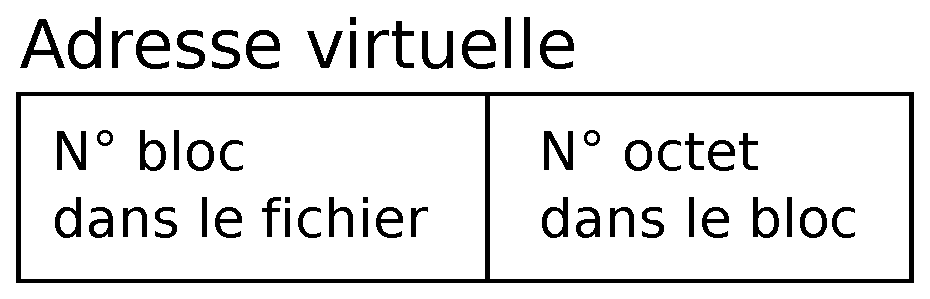
\includegraphics[width=0.5\textwidth]{structure_chainee_temp_adresse_virtuelle}
\end{figure}

Ainsi chaque ligne fait référence à son successeur et son prédécesseur. On stocke également la longueur de l'information («~longueur utile~») et le nombre d'octets disponibles («~longueur max~», supérieure ou égale à la longueur utile) dans l'enregistrement correspondant à une ligne.

La même structure est conservée en mémoire centrale, mais les blocs ne sont pas forcément dans le même ordre \footnote{Cf. page \pageref{subsec:gestionblocs} : «~\nameref{subsec:gestionblocs}~»}. Cela permet de retrouver facilement sur le disque une ligne devant être chargée par la suite.

\begin{figure}[H]
	\centering
	\caption{Structure des données de la solution 3 (exemple)}
	\subfloat[Structure du fichier temporaire]{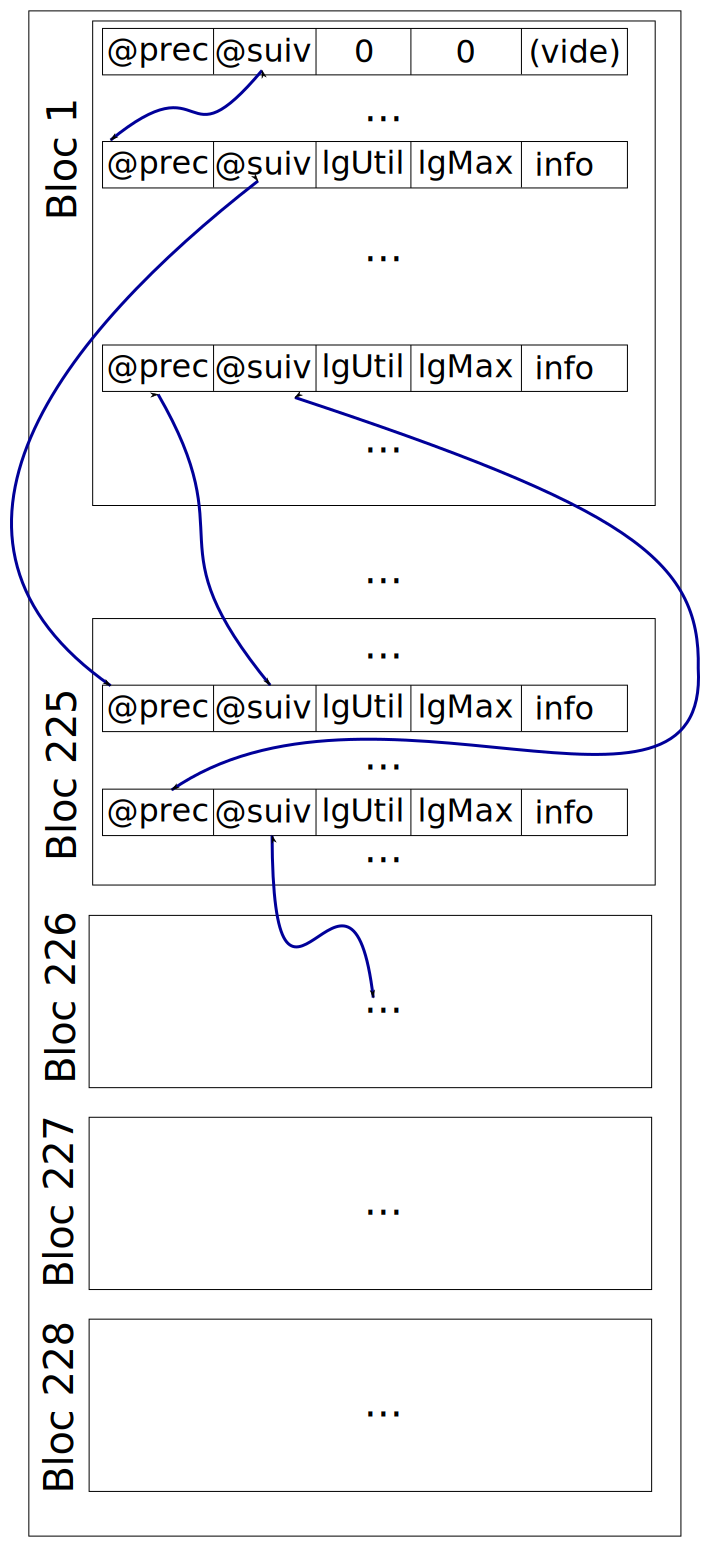
\includegraphics[width=0.4\textwidth]{structure_chainee_temp}}
	\subfloat[Structure du tampon en mémoire centrale]{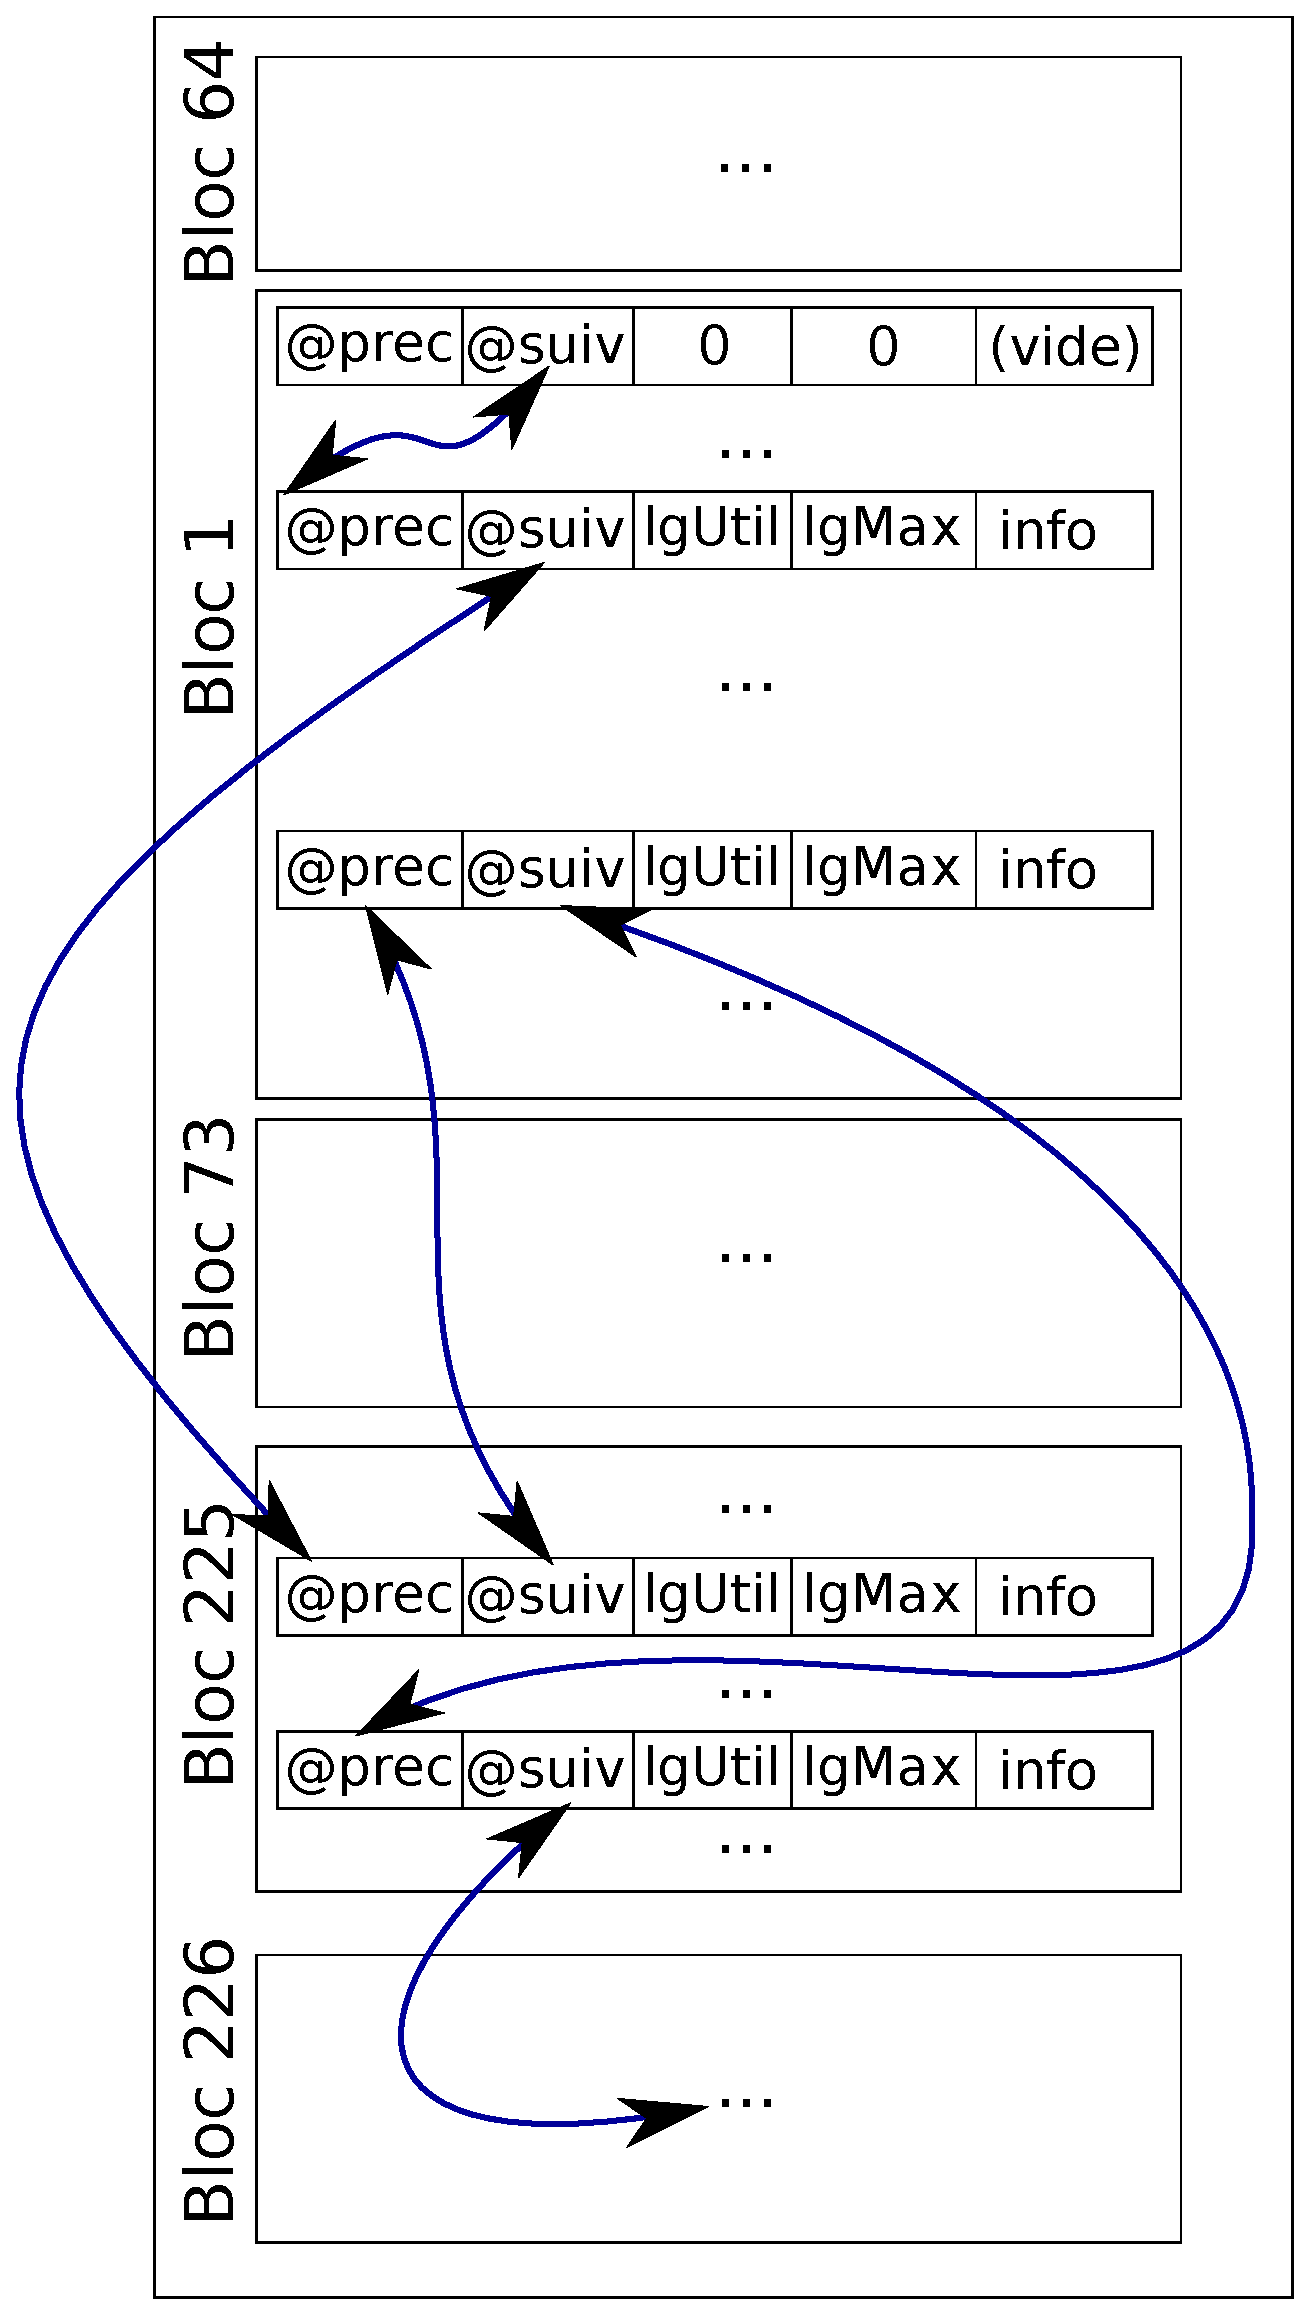
\includegraphics[width=0.4\textwidth]{structure_chainee_mc}}
\end{figure}

\begin{itemize}
	\item Lors d'une insertion, l'algorithme classique d'insertion d'un élément dans une liste chaînée est utilisé. Le nouvel enregistrement est placé au premier espace libre du fichier temporaire quoi soit assez grand pour l'accueillir\footnote{Cf. page \pageref{subsec:gestionespacelibre} : «~\nameref{subsec:gestionespacelibre}~»}, et les adresses concernées (précédente, suivante, suivante de la précédante, précédante de la suivante) sont mises à jour.
	\item Lors d'une modification entraînant un dépassement de la taille maximum de la ligne, on la déplace dans le premier espace libre assez grand pour l'accueillir, et on met à jour les adresses des lignes contigües.
	\item Lors d'une suppression, on met simplement à jour les adresses des lignes contigües afin d'enlever la ligne supprimée du chaînage.
\end{itemize}

On remarquera qu'une ligne «~zéro~» a été ajoutée, ceci pour permettre de généraliser les opérations d'insertion et de suppression de ligne. De même, une ligne de «~fin~» est présente (non représentée sur les schémas). Aucune de ces deux lignes n'est affichée à l'écran.


\subsection{Mécanisme de stockage en mémoire secondaire permettant l'accès direct}
% Yoann

L'accès direct dans le fichier temporaire est possible grâce à la table de \textsl{mapping}, qui donne, pour une partie des lignes, l'adresse virtuelle de celles-ci.

\newcommand{\TableSolTroisHLine}{\cline{1-4} \cline{6-6}}
\begin{table}[H]
	\centering
	\caption{Structure de la table de \textsl{mapping} de la solution 3 (exemple pour $L = 10$)}
	\begin{tabular}{|c|c|}
		N\textdegree{} ligne & Adresse virtuelle \\
		\hline
		\hline
		10 & bloc 226, octet 156 \\
		\hline
		18 & bloc 226, octet 212 \\
		\hline
		25 & bloc 227, octet 61 \\
		\hline
		\multicolumn{2}{:c:}{} \\
		\multicolumn{2}{:c:}{\ldots} \\
		\multicolumn{2}{:c:}{} \\
		\hline
		110 & bloc 54, octet 451 \\
		\hline
		120 & bloc 54, octet 564 \\
		\hline
	\end{tabular}
\end{table}

À la construction du fichier, on mémorise dans cette table l'adresse virtuelle d'une ligne toutes les $L$ lignes ($L$ à définir). La table est indexée par le numéro de ligne.

Lors de l'ajout d'une ligne, la table est mise à jour :
\begin{itemize}
	\item Les enregistrements concernant les lignes suivantes voient leur index incrémenté (le numéro de ligne est mis à jour).
	\item Si la ligne précédant celle insérée dans la table et la ligne suivante ont désormais une différence d'index supérieure à $L$, une ligne est choisie entre les deux pour être insérée dans l'index.
\end{itemize}

Lors de la modification d'une ligne indexée entraînant un déplacement de celle-ci, son adresse dans la table de \textsl{mapping} est mise à jour.

Lors de la suppression d'une ligne indexée, elle est supprimée de la table.\\

Lorsque l'on désire accéder directement à une certaine ligne, il suffit de trouver la ligne la plus proche qui soit indexée dans la table, puis de suivre le chaînage. Grâce aux opérations réalisées à l'ajout d'une ligne, on s'assure de borner (par $0$ et $L$) le nombre de chaînages à parcourir avant de trouver la ligne désirée. L'accès n'est donc pas réellement \emph{direct}, mais il en a les propriétés (la complexité algorithmique constante).

Cette solution permet d'éviter de stocker une entrée dans la table pour chaque ligne, ce qui pourrait se révéler coûteux en mémoire dans le cas d'un très grand fichier. 

Le lecteur attentif aura noté que la table comporte un risque de dégénérescence, si toutes les lignes non indexées sont supprimées : alors toutes les lignes restantes seront indexées. C'est pourquoi on fixera un seuil $Lmin$ : lorsque, à la suite d'une suppression, un index se retrouvera compris entre deux autres dont l'écart d'index est inférieur à $Lmin$, il sera «~désindexé~». 


\subsection{Gestion des blocs sur la mémoire secondaire pour faire de l'accès
    direct et gestion du texte en mémoire centrale}
	\label{subsec:gestionblocs}
% Martin
% COMMENTAIRES - Yoann :
%% Cf. schéma du paragraphe "structuration d'une ligne en mémoire secondaire et en mémoire centrale"
%% Le titre veut rien dire, et il ressemble beaucoup à "Mécanisme de stockage en mémoire secondaire
%% permettant l'accès direct". Je pense qu'il faut dire ici à quel moment on transfère l'information du
%% buffer vers le fichier temporaire et inversement, et comment on gère les blocs actuellement chargés en mémoire tampon.
%% En tout cas il faut le dire quelque part, et ailleurs ça m'a pas l'air de coller.
% Toujours commentaire : Paul
% C'est moi qui ait mis les titres, je les ai copiés du poly.

\subsection{Gestion de l'espace libre}
	\label{subsec:gestionespacelibre}
% Paul
Lorsque beaucoup de modifications ont lieu sur le document actuellement édité,
il peut se produire un phénomène de fragmentation dans la structure de
donnée.

Le phénomène de fragmentation se produit lorsque la taille de l'espace libre
dans les maillons est trop faible pour effectuer une nouvelle insertion dans ce
même maillon (voir page \pageref{sec:structurationligne} pour le procédé
d'insertion). L'espace libre est alors «~perdu~», puisqu'aucun caractère n'y
sera inséré.

Ce phénomène rend de moins en moins efficace la solution technique, par la
même la vitesse du logiciel, et donc finalement l'ergonomie. En effet,
plus la fragmentation est importante, plus le nombre de blocs augmente. De plus,
le nombre d'éléments dans la liste chainée augmente de la même manière, ce
qui augmente le temps de recherche dans la structure de donnée.
Enfin, un nombre plus important de maillons et de bloc signifie aussi une
utilisation mémoire encore plus importante, puisque chaque maillon occupe des
information annexes (pointeurs, informations sur le nombre de caractères
utilisés et libres\ldots).

Il semble donc absolument nécessaire de remédier à ce problème.

Un procédé de défragmentation pourra être appelé, soit manuellement, soit à la
sauvegarde, et reconstruira les structures de données de manière optimale, c'est
à dire de façon à minimiser l'espace non utilisé dans les structures de données.
Une solution pourrait consister à repartir d'un fichier d'un seul bloc et de
reconstruire le double chainage et les adresses virtuelles. La sauvegarde semble
alors être un bon moment pour effectuer cette opération, puisque la «~mise à
plat~» de la structure de donnée sera déjà effectuée pour l'enregistrement sur
disque.



\section{Proposition d'architecture}
% Paul
% Découpage modulaire et hiérarchique
L'architecture choisie sera organisée en couches, afin de découpler le code, et de
permettre une meilleur maintenabilité. On pourrait même imaginer insérer
d'autres couche entre celles présentes dans le tableau ci-dessous, afin de, par
exemple, ajouter facilement un mécanisme d'historique, qui semble intéressant
pour l'édition de code source. Elle se placerait entre la couche interaction
utilisateur et la couche page, sans nécessité pour autant de toucher à ces deux
modules (sauf, bien sur, pour ajouter les nouvelles fonctionnalités dans
l'interface homme-machine).

\begin{center}
    \begin{tabular}{l|p{7cm}}
	Nom de la couche & Description succincte \\
	\hline \hline
	Couche d'interaction utilisateur & Prend en charge l'ensemble de
	l'interaction utilisateur : entrée de commande, et retour visuel.\\
	\hline
	Couche page & Prend en charge le mécanisme de découpage en pages du
	texte chargé.\\
	\hline
	Couche ligne & Prend en charge le mécanisme de découpage en ligne d'une
	page.\\
	\hline
	Couche adressage & Implémente le mécanisme d'adressage virtuel pour
	l'accès direct présenté dans les parties précédentes\\
	\hline
	Couche physique & Prend en charge les appels système pour interagir
	avec le disque.\\
	\hline
    \end{tabular}
\end{center}

Il sera possible de remplacer une couche par une autre, afin d'adapter
l'éditeur à des cas très précis, sans devoir refaire entièrement son
développement. Par exemple, le logiciel pourra être adapté pour des personnes
ne pouvant pas utiliser un clavier, simplement en changeant la couche
d'interaction utilisateur par un module de reconnaissance vocale.


%%%%%%%%%%%%%%%%%%%%%%%%%%%%%%%%%%%%%%%%%%%%%%%%%%%%%%%%%%%%
\section{Bilan}
% Martin
% Bilan de la solution choisie par rapport aux exigeantes + réflexions personnelles
